\chapter{Introduction}

\section{Context}

This thesis is the capstone project of my Master's program between the academic years 2019-2021 in the Media Arts and Sciences program at the MIT Media Lab, where I am a Research Assistant in the Opera of the Future and Future Sketches groups.

This thesis is a collection of media arts instruments made with microcontrollers and \acrfull{ML}, with a strong emphasis on \acrfull{AI} ethics and \acrfull{DIY} methods. Its primary audience - beyond academia - is beginners and artists, and it is my hope that this work can inspire a new generation of instrument makers, artists, designers, educators, programmers, policy makers, activists, and enthusiasts.

\begin{figure}[ht]
  \centering
  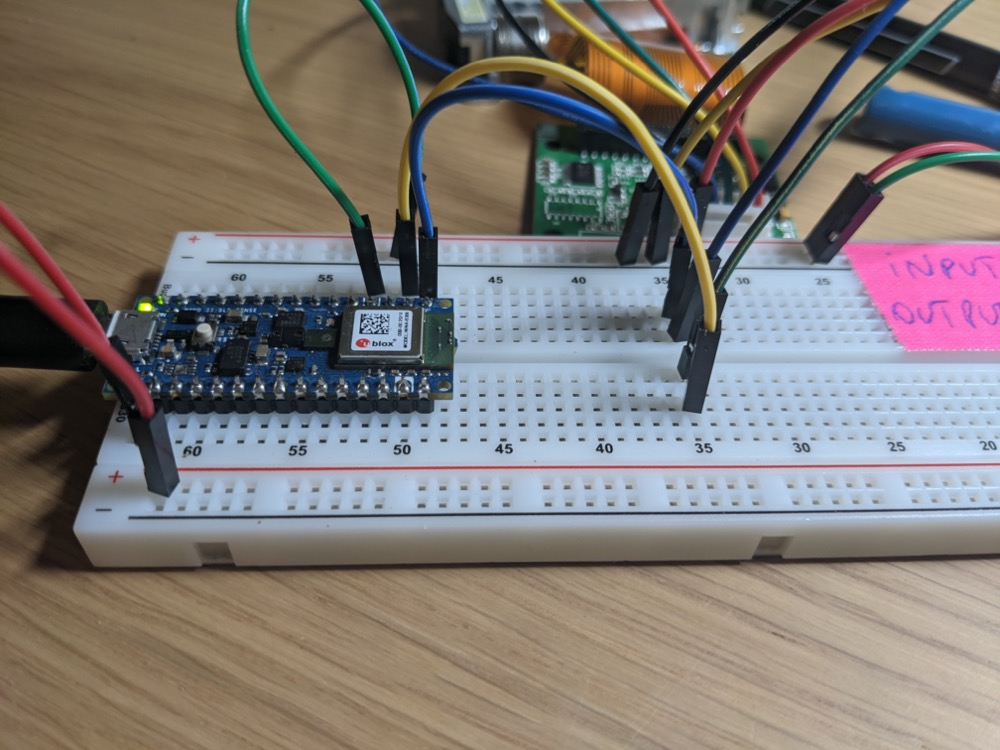
\includegraphics[width=0.75\linewidth,height=0.25\textheight,keepaspectratio]{images/tiny-trainable-instruments-early-protoype.jpg}
  \caption{Early prototype of Tiny Trainable Instruments}
  \caption*{Picture taken by myself}
  \label{fig:tiny-trainable-instruments-early-protoype}
\end{figure}

\acrshort{ML} has several barriers of entry, including cost, complexity, and difficulty. Present day industrial \acrshort{ML} relies on proprietary software and hardware; as a result, \acrshort{ML} models aim for high precision and thus need to be trained for long periods of time, using expensive non-open computational resources, with huge datasets that often are scraped from the internet without the explicit consent of users, and are a byproduct of surveillance capitalism.

\begin{figure}[ht]
  \centering
  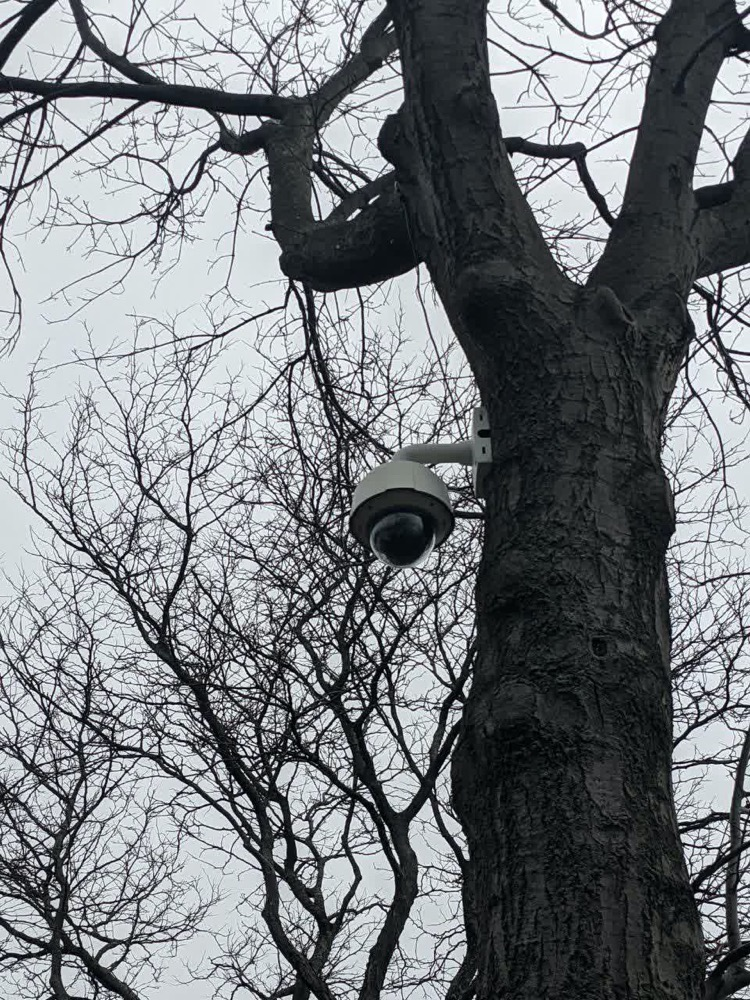
\includegraphics[width=0.75\linewidth,height=0.30\textheight,keepaspectratio]{images/surveillance-camera-tree.jpg}
  \caption{Surveillance camera in a park in Boston MA}
  \caption*{Picture taken by myself}
  \label{fig:surveillance-camera-tree}
\end{figure}

The release of the library Arduino TensorFlow Lite Micro in late 2019 \cite{google-tensorflow-lite-micro-arduino} introduced me to the \emph{tiny \acrshort{ML} field}, a subset of \acrshort{ML} that focuses on hardware and software able to run calculations both on-device and with low power, a stark contrast to many industrial \acrshort{ML} applications. The tutorials published by Arduino \cite{arduino-tensorflow-fruit-identification} showed how to build your own database to detect colors and gestures using a microcontroller, and this was an inspiration to include the same functionalities in this thesis, in order to make an artistic exploration of these emerging techniques.

One aspect that deeply resonated with me was \textbf{data agency}, and being in control of your own data, in particular its capture, storage, publication, and use. In this thesis I propose the microcontroller as a way of building our own databases and deploying our models to bypass corporate or government surveillance. During this year and more of pandemic lockdown context, I have found myself several times working alone in my room, capturing data of myself and my living environment, and then building databases for other people to use, in a way that is reminiscent of one of my favorite artists and activists, Ai Weiwei, who in 2012 - while facing government surveillance - decided to livestream from his house \cite{website-forbes-ai-weiwei-cam}. I also see this today as a way of reclaiming data agency.

\begin{figure}[ht]
  \centering
  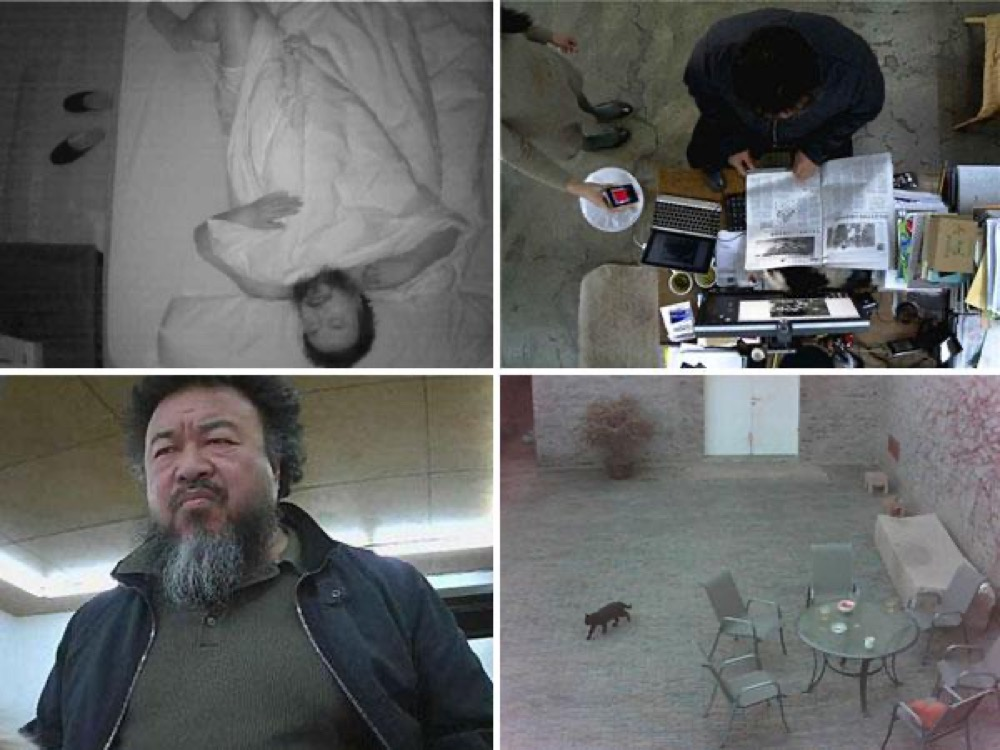
\includegraphics[width=0.75\linewidth,height=0.30\textheight,keepaspectratio]{images/weiweicam.jpg}
  \caption{Weiweicam, by Ai Weiwei, 2012}
  \caption*{Retrieved from \cite{website-forbes-ai-weiwei-cam}}
  \label{fig:weiweicam}
\end{figure}

I am an underrepresented minority in the USA, and it often happens that supposedly automatic neutral technologies fail to detect me. Here is an example of the popular software Zoom, where I spoke out loud: "This is a test to show that Zoom speech to text transcription does not work with my voice because of my accent." Indeed the words "Zoom" and "voice" were transcribed as "soon" and "boys", respectively.

\begin{figure}[ht]
  \centering
  
\includegraphics[width=0.75\linewidth,height=0.25\textheight,keepaspectratio]{images/zoom-introduction.jpg}
  \caption{Screen capture of speech-to-text on Zoom, introduction}
  \caption*{Screen capture by myself}
  \label{fig:zoom-voice}
\end{figure}

Here is a further experiment with more unusual words, the names of the members of my thesis committee: Tod Machover, Mitchel Resnick, and Zach Lieberman, where the transcription had even more errors.

\begin{figure}[ht]
  \centering
  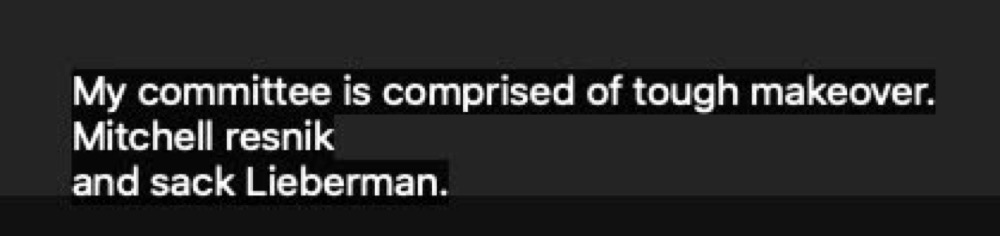
\includegraphics[width=0.75\linewidth,height=0.25\textheight,keepaspectratio]{images/zoom-committee.jpg}
  \caption{Screen capture of speech to text on Zoom, committee}
  \caption*{Screen capture by myself}
  \label{fig:zoom-committee}
\end{figure}

Despite these \acrshort{ML} algorithms being promoted by corporations and governments as unbiased and effective, most probably these algorithms have never been exposed to Chilean people with my accent, so they fail in transcribing my message. Because of these errors, I routinely turn off voice assistants and text completion in my devices (if you have interacted with me over text, I typed every single character :)).

These algorithmic decisions can easily have devastating effects in equity and discrimination. A famous example of this was the scrapped internal recruiting tool that Amazon developed with \acrshort{AI}, which systematically discriminated against women applicants, thus in fact reproducing and amplifying the existing biases of their own hiring teams\cite{website-reuters-news-amazon-ai-bias}. Researcher Timnit Gebru has also published about the dangerous bias and ecological impact of recently released language models \cite{wired-timnit-gebru-google}.

\begin{figure}[ht]
  \centering
  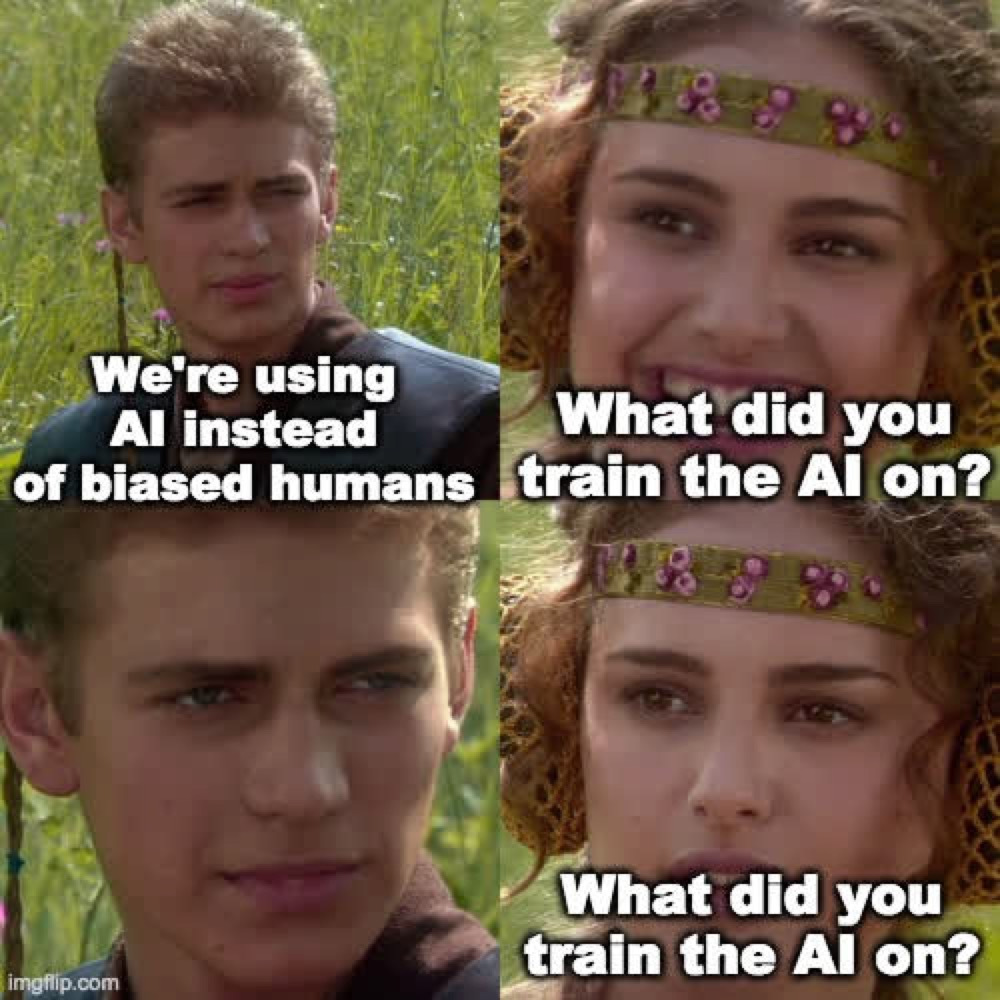
\includegraphics[width=0.75\linewidth,height=0.40\textheight,keepaspectratio]{images/meme-star-wars.jpg}
  \caption{Meme about biased data}
  \caption*{Retrieved from \cite{website-twitter-janellecshane-meme}}
  \label{fig:meme-star-wars}
\end{figure}

Sadly, we often cannot turn off or opt out of these computational or \acrshort{AI} systems. We should in fact be able to, because there is even more at stake than losing our privacy! We could be subjected to harmful \textbf{algorithmic bias}, as the Algorithmic Justice League \cite{website-algorithmic-justice-league} explains on their website:

\begin{displayquote}
"In today’s world, AI systems are used to decide who gets hired, the quality of medical treatment we receive, and whether we become a suspect in a police investigation. While these tools show great promise, they can also harm vulnerable and marginalized people, and threaten civil rights. Unchecked, unregulated and, at times, unwanted, AI systems can amplify racism, sexism, ableism, and other forms of discrimination."
\end{displayquote}

I highly recommend watching the Coded Bias documentary \cite{website-coded-bias} currently available on Netflix, to inform oneself about the important and necessary digital advocacy of the Algorithmic Justice League, who have helped me learn the language for navigating these important topics of civil rights.

The final catalyst that led me to this thesis happened a year ago, when I watched a video \cite{website-talk-technology-and-public-art-rafael-lozano-hemmer} of a conversation between artists Rafael Lozano-Hemmer and Dorothy Santos. At 36:28 in the video, Rafael says "Face recognition needs to be banned in all applications except art."

This was the perfect spark for starting to work on this project, inspiring me to make more accessible these computational techniques to artists, beginners, enthusiasts, and educators. I think it's crucial for our civil rights and advancing the discourse, that artists experiment with \acrshort{ML} in a critical way. Despite the creative and artistic applications that I show in this thesis, and how \acrshort{ML} becomes cheaper and more pervasive, it is not the solution to all problems, and might not even be needed in many scenarios.

\begin{figure}[ht]
  \centering
  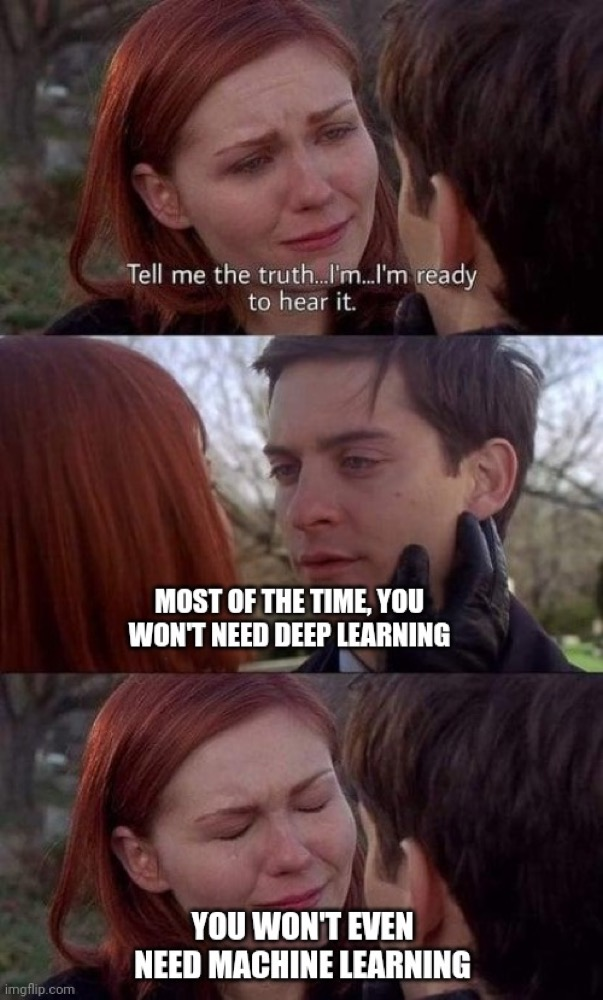
\includegraphics[width=0.75\linewidth,height=0.50\textheight,keepaspectratio]{images/meme-spider-man.jpg}
  \caption{Meme about need of machine learning}
  \caption*{Retrieved from \cite{website-twitter-dynamicwebpaige-meme}}
  \label{fig:meme-spider-man}
\end{figure}

In this 21st century, artists have unprecedented access to tools for making more new tools and instruments, and I intend this thesis to be a foundation for a new generation of instrument makers for manipulating audiovisual material, using \acrshort{ML}. This approach is really exciting because it allows beginners and artists to train their instruments instead of programming them, by inputting data for tuning instead of having to write lines of code, and then fixing thresholds for changing their behavior, working off-the-cloud in a decentralized way.

This thesis project main contribution is wrapping the recent advances of industrial \acrshort{ML} running on microcontrollers with the discourse on ethical \acrshort{AI}, into an user-friendly software and hardware packaging. Tiny Trainable Instruments is a holistic project, including all the steps to build your own \acrshort{ML}-enabled arts instruments: from using sensors to create your own custom databases to train your small-scale \acrshort{ML} models, to deploying them with privacy-preserving practices to your microcontrollers and different multimedia outputs.

\section{Objectives and dreams}

Infrastructure and cooperation are key to society. I love how I can bike on roads and hike on paths that were built as shared resources for the benefit of everyone. I hope this thesis work can be adopted by fellow artists and educators to create new instruments for arts, and to inspire critical and ethical thinking about \acrshort{AI}.

There is a significant educational value in creating your own databases, and in this thesis I propose techniques and software so that people can do this. By building databases with their own data, people will be able to train their own custom \acrshort{ML} models that are tailored to themselves, instead of using external databases and inheriting their biases. Also I hope this work will help people appreciate the craft involved in making databases, and raise awareness about the exploitation and problematic lack of consent behind them.

Finally, I want to highlight all the legal documents and regulations that I navigate on a daily basis: as a non-U.S. citizen on a student visa I cannot freelance, as a software programmer I have to comply with various licenses, and as a musician I am still learning about the different ways to publish covers and to sample other artists. Some of the most pervasive documents that we encounter are the terms and conditions of the services we use. As an anecdote, in 2010, GameStation added a soul clause to theirs as an April Fool's prank, making them legal owners of thousands of customers' souls \cite{website-huffpost-gamestation-soul-clause}. A study in 2007, it was estimated that people would need around 250 hours every year to actually read the privacy policies shown to them \cite{article-cost-of-reading-privacy-policies}. That is why in this thesis I have tried my best to cite every work that I am either using as a building block, or that served as a direct or indirect inspiration.

I hope this work can be adopted and iterated on by others, through building a new generation of private and smart devices, like one of my first goals, a drum machine I can talk to, and that would let me ask for different rhythms mid-performance, or let me use my body gestures to write poems.

\section{Thesis outline}

\begin{enumerate}
  \item Chapter 1 - Introduction: the context and summary.
  \item Chapter 2 - Early experiments: media arts education, microcontrollers, and \acrshort{ML}, among others.
  \item Chapter 3 - Background and inspiration: research about work by other people which has informed my practice.
  \item Chapter 4 - Tiny Trainable Instruments: design strategies for the software and hardware, description of the support team working on this thesis.
  \item Chapter 5 - Project evaluation: user feedback, field notes.
  \item Chapter 6 - Conclusions and future work: next iterations of the instruments, and their proposed use for educators and artists.
  \end{enumerate}
